\documentclass[12pt,a4paper]{article}
\usepackage[utf8]{inputenc}
\usepackage{amsmath}
\usepackage{amsfonts}
\usepackage{amssymb}
\usepackage{makeidx}
\usepackage{graphicx}
\usepackage[left=2cm,right=2cm,top=2cm,bottom=2cm]{geometry}
\parindent=0cm %modificar tamaño de sangria 
\usepackage{epstopdf}
\usepackage{float}
\usepackage{subfigure}
\usepackage{array}
\newcolumntype{E}{>{$}c<{$}}
\usepackage{longtable}

\begin{document}
\title{\textbf{Sistemas electronicos de interfaz\\Reporte final\\P.I.S.T.O.}}
\author{Alvarez Hernandez Edwin David 18311619\\Arce Montaya Jonathan 18311603\\Briano Garcìa Angel Eraclio 18311625\\Bueno Gòmez Jorge Heriberto 18312259\\Cruz Cervantes Oscar 18311638\\Orozco Nevares Josue Natanael 18311797\\Lisbeth Martinez Velazquez}
\date{8 de noviembre del 2019}

\begin{figure}
\centering

\includegraphics[width=10cm]{UPCDLZMDG5783-logo.png} 
\end{figure}
\maketitle
\newpage

\section{Portador inteligente servicial para tomadores organizados (P.I.S.T.O.)}

\section{Problematica}
Vasos preparados erroneamente de manera manual debido a el mal manejo de las materias primas para preparar dichas bebidas.

\section{Problema a resolver}
Al realizar la investigacion se determina el problema a resolver, el cual es hacer una distribucion casi perfecta de alcohol en bebidas preparadas (alcoholicas).\\
En la recoleccion de informacion y evidencias notamos que el alcohol se desperdicia en pequenas proporciones que al pasar el tiempo en el evento es una perdida de producto y de dinero.\\
Las razones por la que sucede son diversas, descuidos, vasos con demasiado alcohol y por lo tanto lo dejan de beber o lo tiran, caidas, etc\\El problema por el cual nos vamos a inclinar a resolver sera:\\El suministro adecuado en cada bebida preparada.\\El control y proteccion de las bebidas alcoholicas (para evitar accidentes).\\Un servicio comodo y sencillo de utilizar.\\Rapidez en el servicio.


\section{Objetivo general}
Preparar bebidas lo mas exactas para cada tipo de persona que desee beber alcohol acorde a su gusto.

\section{Objetivos especificos:}
1. Proponer ideas para llevar acabo el proyecto\\2. Diseñar el boceto para ver que necesitamos\\3. Analizar los compotentes que necesitamos.\\4. Comprar los componentes.\\5. Elaborar el proyecto.\\6. Elaborar el programar del plc.\\7. Determinar las pruebas correspondientes.\\8. Analizar si hubo algun error.\\
\section{Justificacion}
Este proyecto es realizado por la necesidad de facilitar y mejorar procesos de llenado con una mayor precisión, velocidad, y un aumento de la producción, además de reducir los accidentes, perdidas y costos.

\subsection{Delimitacion}
1- Servir entre 10 y 20 vasos\\
2- Preparar un tipo de bebida a la vez.\\
3- Unicamente el proyecto contara con tres tolvas para cargarlas con los liquidos y seran: el tipo de alchol con el que se deseen preparar las bebidas, agua mineral al gusto y finalmente refresco que va acorde con el alcohol para mejor sabor y disfrute del usuario.
4- El hielo se tendra que colocar manualmente.

\section{Costos}
\begin{table}[H]
\centering
\begin{tabular}{|m{3.5cm}|m{3.5cm}|m{3.5cm}|m{3.5cm}|}
\hline

Cantidad  & Material o componente  & Precio unitario & Precio total\\
\hline
1 & Sensor de flujo yf-s201 & 150 & 150\\
\hline
1 & Display LCD 16X2 HD44780 / 100 & 100\\
\hline
1 & Modulo relevador de 4 canales & 115 & 115\\
\hline
2 & Válvula Solenoide 12 Vcd Nc 1/2 & 150 & 300 \\
\hline
2 & Mini Bomba De Agua 12v 6w R385 & 220 & 440 \\
\hline
2 &  Módulo sensor laser ky-008 & 40 & 80 \\
\hline
1 & Raspberry Pi3 B+ & 1150 & 1150 \\
\hline 
1 & Motor 110v & 1600 & 1600 \\
\hline
- & Materiales de construcción & 1500 & 1500 \\
\hline
- & Extras & 500 & 500\\
\hline
- & - & Total & 5935\\
\hline



\end{tabular}
\caption{Costos estimados para el proyecto}
\label{lineas}
\end{table}
\section{Matriz de roles}
\begin{tabular}{|c|c|}
\hline 
Signo  & Leyenda  \\ 
\hline 
P & Responsabilidad \\ 
\hline 
C & colabora \\ 
\hline 
I & Suministra información a los demás  \\ 
\hline 
NJ & Josué Natanael Orozco Nevares y jonathan Arce Montoya  \\ 
\hline 
EO & Edwin David Álvarez Hernández y Oscar Cruz Cervantes  \\ 
\hline 
BL & Ángel Eraclio Briano García y Lisbeth Martínez Velásquez \\ 
\hline 
\end{tabular} 

\begin{tabular}{|c|c|c|c|c|}
\hline 
Actividades  & NJ & EO & BL & Fecha  \\ 
\hline 
Título del proyecto  & P & I C & C & del 16 al 20 de Sep. 2019 \\ 
\hline 
Planteamiento del problema  & P & I C & C I & del 16 al 20 de Sep. 2019 \\ 
\hline 
Formular el problema  & C & P I & C I & del 16 al 20 de Sep. 2019 \\ 
\hline 
Objetivo general del proyecto  & P & I C & C & del 16 al 20 de Sep. 2019 \\ 
\hline 
Objetivo del proyecto  & C & P I & I C  & del 16 al 20 de Sep. 2019 \\ 
\hline 
Justificación  & C & P I & C & del 16 al 20 de Sep. 2019 \\ 
\hline 
Delimitación & P & I C & I C & del 16 al 20 de Sep. 2019 \\ 
\hline 
Matriz de posibles costos de materiales  & C & I P  & C & del 16 al 20 de Sep. 2019 \\ 
\hline 
Matriz de roles  & C & I & P & del 16 al 20 de Sep. 2019 \\ 
\hline 
Diagrama de Gantt  & C & I & P & del 16 al 20 de Sep. 2019 \\ 
\hline 
Explicación de la aportación de cada materia  & P & I C & C & del 16 al 20 de Sep. 2019 \\ 
\hline 
Desarrollo del proyecto  & P & I & C & del 16 al 20 de Sep. 2019 \\ 
\hline 
Bibliografías  & P C & I & C & del 16 al 20 de Sep. 2019 \\ 
\hline 
Total P & 7 & 4 & 2 & - \\ 
\hline 
Total C & 7 & 5 & 11 & - \\ 
\hline 
Total I & - & 13 & 4 & - \\ 
\hline 
\end{tabular}

\section{Diagrama de Gantt}
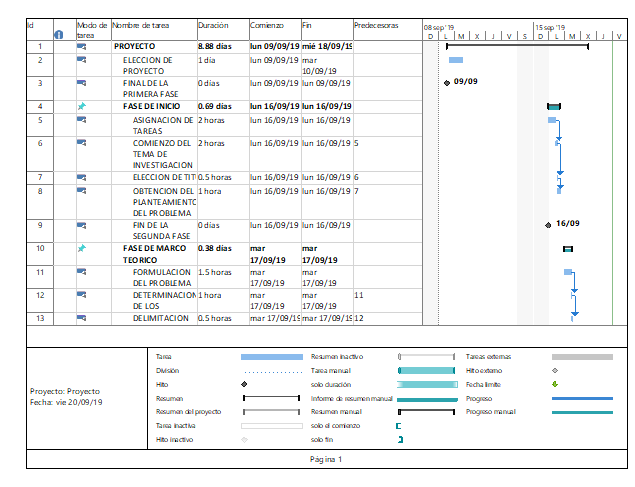
\includegraphics[width=18cm]{Diagrama.png}
\newpage

\section{Materias relacionadas}
\begin{table}[H]
\centering
\begin{tabular}{|m{4cm}|m{11cm}|}

\hline
Materia & Aportación de la materia \\
\hline
Ingles lV &  Lograr entender el nombre de algunos de los materiales de construcción para la máquina, además de al momento de programar se utilizan por lo general comandos en inglés y gracias a esta clase es más entendible cada una de esas palabras.\\
\hline
Ética profesional & Comunicarse con los compañeros de equipo de una manera profesional al momento de aportar ideas u o comentarios acerca del proyecto y su vez tratar de manera profesional a los proveedores que se eligieron para el proyecto y puede que siendo así se llegue a conseguir un beneficio extra de parte de ellos.\\
\hline
Estructura y propiedades de los materiales & Conocer materiales resistentes y adecuados para la construcción del proyecto P.I.S.T.O. \\
\hline
Programación de periféricos & Integrar correctamente cada sensor o acoplamiento que se requiera al cuerpo del proyecto, el cual en este caso será una banda transportadora, a partir de allí se le acoplara lo necesario de una manera eficiente. Inclusive por medio de un PLC. \\
\hline
Sistemas electrónicos de interfaz & Con los conocimientos de la materia se podrá crear una mejor para la creación del proyecto así como su estructura aplicando técnicas de medición en cuanto a nuestras entradas y salidas del proyecto, así como saber que agregar al mismo o simplemente descartarlo\\
\hline
Controladores lógicos programables & Programar cada intervalo de la maquina por medio de tiempos y medidas que se le añadirán al momento ir construyendo cada parte de la banda. Inclusive por medio de un PLC o la configuración de una Raspberry.\\
\hline

\end{tabular}
\caption{materias de 4to cuatrimestre}
\label{lineas}
\end{table}

\begin{table}[H]
\centering
\begin{tabular}{|m{4cm}|m{11cm}|}

\hline
materia & aportación de la materia \\
\hline
Ingles V &  Aportará un mejor manejo del idioma con el cual tendremos más opciones de configuraciones e idiomas en el programa \\
\hline
Habilidades organizacionales & Aportará una habilidad para llevar a cabo nuestras actividades programadas, además de proporcionar un control y organización de nuestro proyecto \\
\hline
Analisis de mecanismos & En esta material podremos mejorar nuestro Sistema, aprendiendo un poco más sobre las funciones de mecanismos y genera un mejor criterio en la toma de decisiones y desarrollo de nuestro proyecto \\
\hline
Sensores y acondicionamiento de señales & En esta materia aprenderemos a utilizar sensores y ya que nuestra maquine necesita medidas con este conocimiento podremos mejorar nuestro sistema de llenado \\
\hline
Microcontroladores & Con esta materia veremos las funciones y usos de dichos dispositivos los cuales nos ayudaran a controlar nuestra máquina.\\
\hline
Moldeado y simulación de sistemas & En esta materia nos ayudara a mejorar nuestro diseño para poder detectar posibles errores antes de para a ensamblar los componentes necesarios \\
\hline
Mecánica de flujos & Esta materia aportara algo muy importante ya que podremos comprender como se comporta el alcohol con el que estaremos trabajando y así controlar sus propiedades para un funcionamiento más óptimo de nuestra maquina \\
\hline

\end{tabular}
\caption{materias de 5to cuatrimestre}
\label{lineas}
\end{table}

\begin{table}[H]
\centering
\begin{tabular}{|m{4cm}|m{11cm}|}

\hline
Ingles Vl & Esta materia aportara un mejor dominio del idioma con el cual podremos hacer un menú en ingles de la maquina.\\
\hline 
Ética profesional & En esta materia aprenderemos los valores que nos ayudara a generar un mejor entorno al estar trabajando en equipo. \\
\hline
Diseño mecánico & esta materia nos explicara más a fondo el sistema mecánico para poder desarrollar nuestro proyecto y poder evitar la mayor cantidad de falla posibles. \\
\hline
Automatización industrial & en esta materia nos ayudara a ver el proceso de automatización para poder implementarlo en nuestra máquina, será muy importante ya que este tema nos ayudara a mejorar nuestro sistema y a detectar errores en el ámbito de la automatización \\
\hline
Maquinas eléctricas & En esta materia aprenderemos el uso correcto de la maquinas eléctricas y podremos aprovechar al máximo este tipo de recursos \\
\hline
Procesos de manufactura & En esta materia comprenderemos lo procesos que se llevan a cabo en manufactura y podríamos diseñar y proyecto más grande y llevarlo a distintos tipos de tiendas y empresas (pero eso estaría por ver)\\
\hline
Sistemas hidráulicos y neumáticos & Con esta materia podremos aprender que tipo de sistema se acopla mejor a nuestro proyecto y de esa manera poder trabajar con él.\\
\hline 

\end{tabular}
\caption{materias de 6to cuatrimestre}
\label{lineas}
\end{table}

\section{Desarrollo}
El desarrollo del proyecto a ido progresando exponencialmente a lo largo de este periodo cuatrimestral, destacando las areas de estudio y apoyo en la cual se a basado nuestro proyecto, refiriendonos a las materias impartidas, por ejemplo:

\subsection{Ingles V}
Gracias a esta materia a sido posible identificar materiales necesarios y componentes de mayor calidad debido a que la mayoria de estos componentes vienen de origen estadounidense.

\subsection{Ètica profesional}
Lograr resolver problemas en el equipo dialogando acerca de los mismo y la organizaciòn adecuada para la construcciòn de este proyecto repartiendo equitativamente los deberes.

\subsection{Estructura y propiedades de los materiales}
Conocimiento adecuado de las sustancias y materiales a necesitar en el proyecto.

\subsection{Programaciòn de perifèricos}
Diseñar el codigo de funcionamiento para el PLC que se le acoplara en el futuro a P.I.S.T.O.

\subsection{Sistemas electrònicos de interfaz}
Diseñar una interfaz adecuada para el usuario que desee interactuar con P.I.S.T.O. Siendo asi sencilla y entendible, sin causar problemas al momento de utilizarlo.

\subsection{Controladores lògicos programables}
Acoplar el PLC a P.I.S.T.O. para su funcionamiento autonomo sin dañar el proposito del mismo.\\

\subsection{Materiales reunidos}
Ademas de lo mencionado, se han adquirido partes para la construcciòn del proyecto, los cuales son:\\
\\
\newpage

PLC
\begin{figure}[h!]
\centering
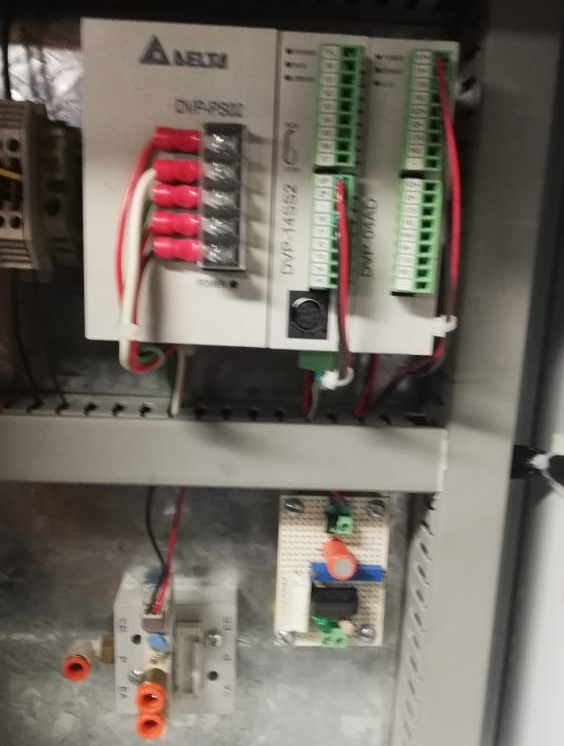
\includegraphics[width=8cm]{PLC.jpg} 
\end{figure}

Motor
\begin{figure}[h!]
\centering
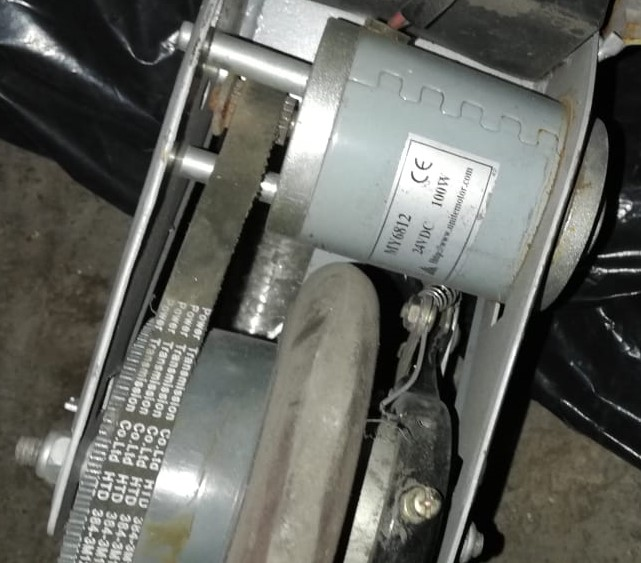
\includegraphics[width=8cm]{Motor.jpg} 
\end{figure}
\newpage

Se construyo un modelo CAD para la visualizaciòn del prototipo del proyecto P.I.S.T.O.

\begin{figure}[h!]
\centering
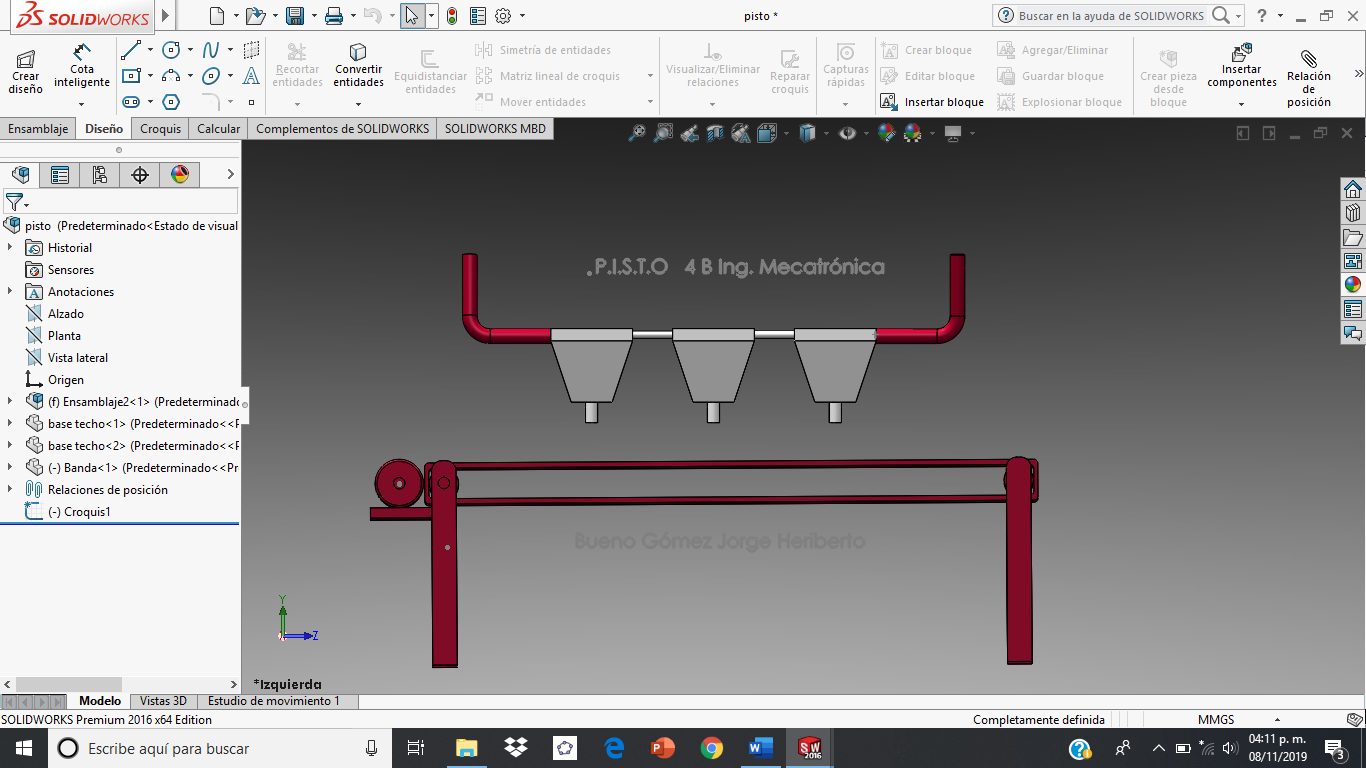
\includegraphics[width=15cm]{img.png} 
\end{figure} 
\newpage
\section{Conclusiones}
\title{\textbf{Alvarez Hernandez Edwin David}}\\

\title{\textbf{Arce Montoya Jonathan}}\\
En el corto periodo de tiempo, fue necesario adaptar los conocimientos adquiridos durante nuestras clases y materias impartidas, la asignatura que tuvo más impacto en nuestro proyecto fue la asignatura de controladores lógicos programables o PLC, ya que el proyecto fue pensado para automatizarlo y nos enfocamos en las ventajas y oportunidades que nos pueden otorgar el sistema de PLC, aún nos hace falta afinar detalles en el proyecto, pero con las nuevas asignaturas y conocimientos que podemos adquirir, esperamos tener ideas mas estructuradas para la mejora y el avance de nuestro proyecto.\\
\title{\textbf{Briano Garcia Angel Eraclio}}\\
Para este Proyecto se tuvo que emplear el conocimiento que adquirimos en el transcurso del cuatrimestre desde la programación y creación de los circuitos, hasta el armado de los 
PCB para el funcionamiento de nuestro proyecto, incluso también se implementó un diseño realizado en formato CAD. Todo esto para beneficio y eficacia del proyecto P.I.S.T.O.\\ 
\title{\textbf{Bueno Gòmez Jorge Heriberto}}\\
En este proyecto encapsulamos muchos conocimientos de las materias de este cuatrimestre, 
como fue la realización de programas para PLC, el diseños y programación de sistemas de interfaz y, también la implementación de circuitos además incluimos conocimientos de otros cuatrimestres como fue el desarrollo del proyecto en un cad.\\
\title{\textbf{Cruz Cervantes Oscar}}\\
En este proyecto se utilizaron los conocimientos adquiridos en el transcurso del cuatrimestre, tomando en cuanta cadauna de las materias aunque dando prioridad a ciertas materias que tienen un mayor aporte que otras, con estos conocimientos adquiridos pudimos hacer un avance significativo en el desarrollo y planificasi`on del pryecto, aunque aùn es muy proto para buscar un producto terminado. \\
\title{\textbf{Orozco Nevares Josue Natanael}}\\
Este proyecto se podria ver como algo chusco pero a fin de cuentas cumple con su fin, el aprender acerca de la elaboraciòn de un sistema automatizado, a pesar de que en este cuatrimestre por lo pequeño que es no se alcanzo a armar en si algo, pero se logro reunir algunos de los componentes base para el proyecto, me hubiese gustado tener mas tiempo para la elaboraciòn del mismo.\\
\title{\textbf{Lisbeth Martinez Velazquez}}\\
El analizar este proyecto, hemos observado lo importante que es implementar y automatizar un sistema para ver las necesidades que se presentan en cada momento.
El tener un analisis es de mucha importancia, ya que implementamos los conocimientos basicos de este cuatrimestre (plc, programacion, electronica, sotware).
En estos dos cuatrimestres que se acercan, seguira el desarrollo, observaremos nuevas mejorias y nuevas automatizaciones para desarrollar y cumplir con el objetivo de ayudar en una necesidad con nuestros conocimientos precios y realizando un proyecto anual.\\
\newpage
\nocite{*}
\bibliographystyle{apalike}
\bibliography{biblio}


\end{document}